\chapter{Zusammenfassung und Ausblick}

Es wurden zwei Verfahren für die 3D-Modellgenerierung von Baumstrukturen vorgestellt:

\paragraph{Lindenmayer-Systeme}

Lindenmayer-Systeme stellen eine Erweiterung von kontextfreien Grammatiken dar, welche Teile einer übergebenen Zeichenkette anhand festgelegter Regeln durch andere Zeichenketten ersetzen. D0L-Systeme, die fundamentalste Form der L-Systeme, werden zu parametrischen L-System erweitert. \cite[S.3]{ABOP:04} Dies ermöglicht die Ableitung von komplexen Zeichenfolgen, welche mithilfe der vorgestellten, grafischen Interpretation von L-System-Resultaten visuell repräsentiert werden. Diese sogenannte Turtle-Interpretation wird für die Verwendung im dreidimensionalen Raum erweitert und and die 3D-Modellgenerierung von Baumstrukturen angepasst. \cite[S.7, 18f, 21ff, 51ff]{ABOP:04}

\paragraph{Space Colonization Algorithmus}

Der vorgestellte Space Colonization Algorithmus basiert auf dem biologisch motivierten Konkurrenzverhalten um Wachstumsraum zwischen wachsenden Ästen eines Baumes. Es werden Punkte in einem festgelegten Bereich generiert, welche die Verfügbarkeit von Wachstumsraum repräsentieren und in jeder Iteration des Algorithmus das Wachstum der Äste beeinflussen. Nähert sich ein Ast einem der Punkte, wird dieser entfernt, um zu signalisieren, dass in diesem Bereich kein Wachstumsraum mehr verfügbar ist. \cite[S.2f]{SpaceColonizationAlgorithm:07} Die Verteilung der Einflusspunkte und das Wachstumsverhalten des Baums in jeder Iteration kann durch Übergabe von numerischen und Boolschen Parameterwerten gelenkt werden. \cite[S.5]{SpaceColonizationAlgorithm:07} 

Weiterhin wurden Erweiterungen des ursprünglichen Algorithmus vorgeschlagen, welche das Wachstumsverhalten beeinflussen, die Generierungszeit verkürzen und zu einer verminderten Datenmenge des generierten 3D-Modells beitragen können.

\paragraph{Implementierung und Ergebnisse}

Die innerhalb der Unreal Engine 4 umgesetzte Implementierung und damit verbundene Visualisierung beider Vorgehen wurde vorgestellt. Über die visuelle Editoroberfläche werden den implementierten Unreal-Actors die jeweils benötigten Parameterwerte übergeben. Beide Verfahren bauen einen graphentheoretischen Baum auf, der von dem implementierten Modellgenerierungssystem zu 3D-Modelldaten verarbeitet und mithilfe des bereitgestellten Grafiksystems dargestellt wird.

Der Einfluss übergebener Parameter auf die generierte Baumstruktur wird behandelt. Definitionen von L-Systemen können sich an dem Verzweigungsverhalten realer Pflanzen orientieren, um realistische Ergebnisse zu liefern. \cite[S.51ff]{ABOP:04} Die verschiedenen Parameter des Space Colonization Algorithmus können mit bestimmten Wachstumsmustern von Bäumen in Zusammenhang gesetzt werden, um komplexe Baumstrukturen zu generieren. \cite[S.5]{SpaceColonizationAlgorithm:07}

\section{Bewertung und Vergleich der Ergebnisse}

Es wurden zwei sich ergänzende Verfahren gewählt, um eine Vielfalt verschiedener Baumstrukturen generieren zu können. Diese Verfahren unterscheiden sich in Hinsicht auf die visuellen Ergebnisse, die Effizienz bei der Anwendung und ihrer Benutzerfreundlichkeit.

\subsection{Visuell}

Der Space Colonization Algorithmus kann insbesondere für die Darstellung der unregelmäßigen Form von Laubbäumen aus den gemäßigten Breiten verwendet werden. Auch ohne die Ergänzung durch Blätter oder Blüten besitzen die sich ergebenden Baumstrukturen eine realistische Form. Die Funktionsweise des Algorithmus stellt sicher, dass keine Überschneidungen von Zweigen stattfinden und ermöglicht eine Anpassung der Baumstruktur an einschränkende Bedingungen hinsichtlich des Wachstumsraumes. \cite[S.5]{SpaceColonizationAlgorithm:07}

Es ist jedoch schwer andere Sorten von Bäumen, wie Nadelhölzer oder tropische Bäume, mit einem klar definierten Stamm und tragenden Ästen darzustellen. Die Einführung des gewichteten Wachstums stellt einen Ansatz für die Generierung solcher Baumsorten dar -- Abbildung \ref{subfig:SCA_GewWachstum_On} zeigt ein Beispiel für eine Tannenbaum-ähnliche Struktur. Diese Erweiterung liefert jedoch nur unter einer Vielzahl von Bedingungen visuell ansprechende Ergebnisse.

L-Systeme bieten eine größere Kontrolle über die generierten Baumstrukturen und erlauben die Simulation natürlicher Wachstumsmuster -- unter anderem ist die Generierung von Baumsorten möglich, die mithilfe des Space Colonization Algorithmus nur schwer oder überhaupt nicht generierbar sind. Durch die Anpassung von Konstanten können mithilfe derselben L-System-Definition sich visuell stark unterscheidende Baumstrukturen erstellt werden. Da die Generierung der Modelle jedoch strikt nach den festgelegten Regeln abläuft, sind in manchen Fällen bestimmte Muster und Regelmäßigkeiten in der Baumstruktur erkennbar, was den Modellen eine unnatürliche Wirkung verleiht. Ein solcher Eindruck kann durch die Anpassung von Konstanten und die Verwendung eines Tropismus-Einflusses reduziert werden, erlaubt jedoch nicht dieselben, unregelmäßigen Formen, die mithilfe des Space Colonization Algorithmus möglich sind. \cite[S.6]{SpaceColonizationAlgorithm:07}

\subsection{Effizienz}

Da L-Systeme auf Grundlage der Ersetzung von Zeichenketten arbeiten, besteht ein Großteil der Generierungszeit des L-System-Actors aus der Konstruktion des graphentheoretischen Baumes durch die Turtle-Interpretation und die darauf folgende Berechnung der Vertexdaten durch das Modellierungssystem. Dies erlaubt eine vergleichsweise schnelle Generierung von komplexen 3D-Modellen. Selbst Modelle mit mehreren Millionen Vertizes -- einer Datenmenge die in Echtzeitanwendungen normalerweise nicht für einzelne Modelle benötigt wird -- werden auf einem Desktop-Computer mit $3.3GHz$-Prozessor in wenigen Sekunden erstellt.

Der Nachteil ist jedoch, dass für die Darstellung einer realistisch wirkenden Baumstruktur durch ein L-System, ohne dass die Aststruktur größtenteils von Blättern verdeckt wird, eine vergleichsweise große Menge Modelldaten benötigt wird. Die vorgestellte Kurvenreduktion kann angewandt werden, hat jedoch kaum Auswirkungen auf die Datenmenge, da sowohl Astsegmente als auch Verzweigungen in den Produktionsregeln definiert und somit nicht auf eine automatische Kurvenreduktion angewiesen sind.

\begin{figure} [hbtp]
	\centering
	\begin{subfigure}[t]{.45\textwidth}
		\centering
		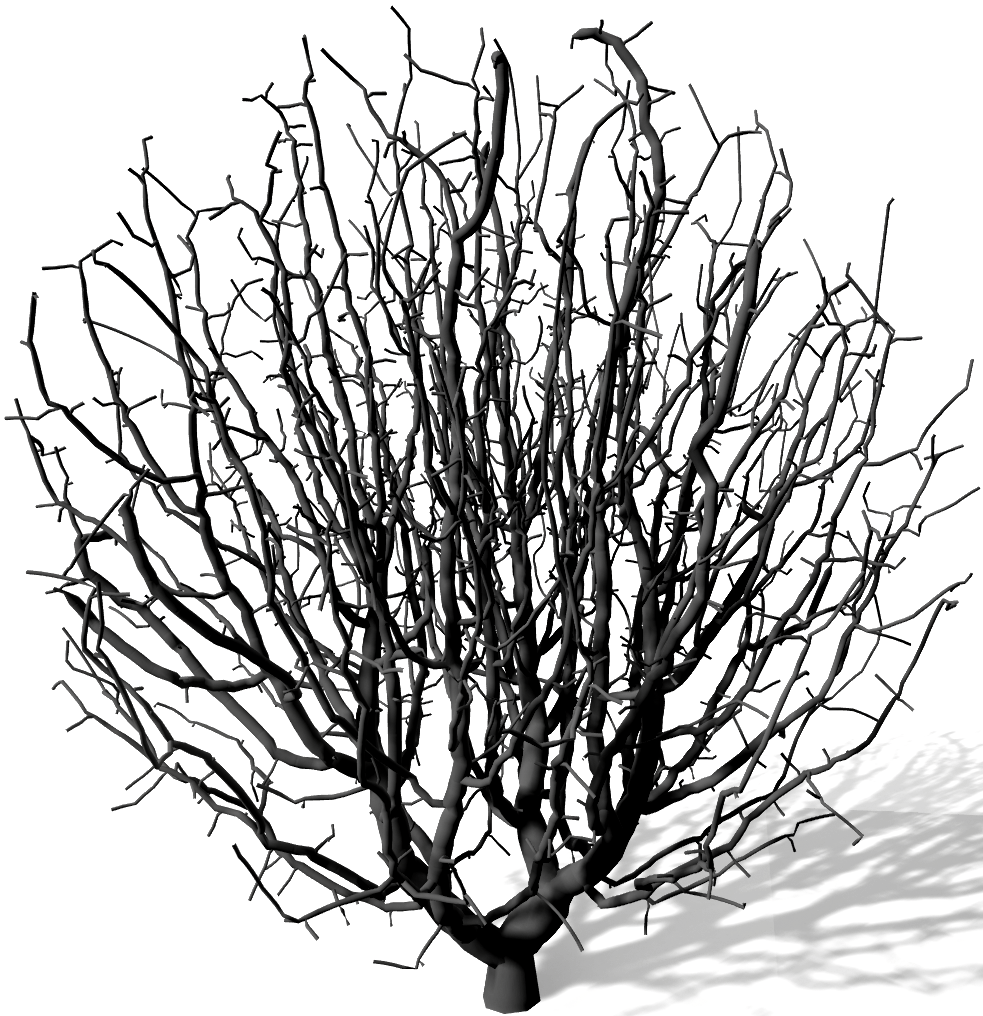
\includegraphics[height=.19\textheight]{images/Performance_SCA_Quali_Segments_High.png}
		\caption{$N = 5000$, $D = 20.0$, $N_I = 1000$,\\ $n_{min} = 8$, $n_{max} = 8$, $max_K = 1.0$,\\  $\text{Generierungszeit} = 2.416s$, $103725 \text{ Vertizes}$.}
		\label{subfig:Performance_SCA_Quali_Segments_High}
	\end{subfigure}
	%\hspace{.05\linewidth}
	\begin{subfigure}[t]{.5\textwidth}
		\centering
		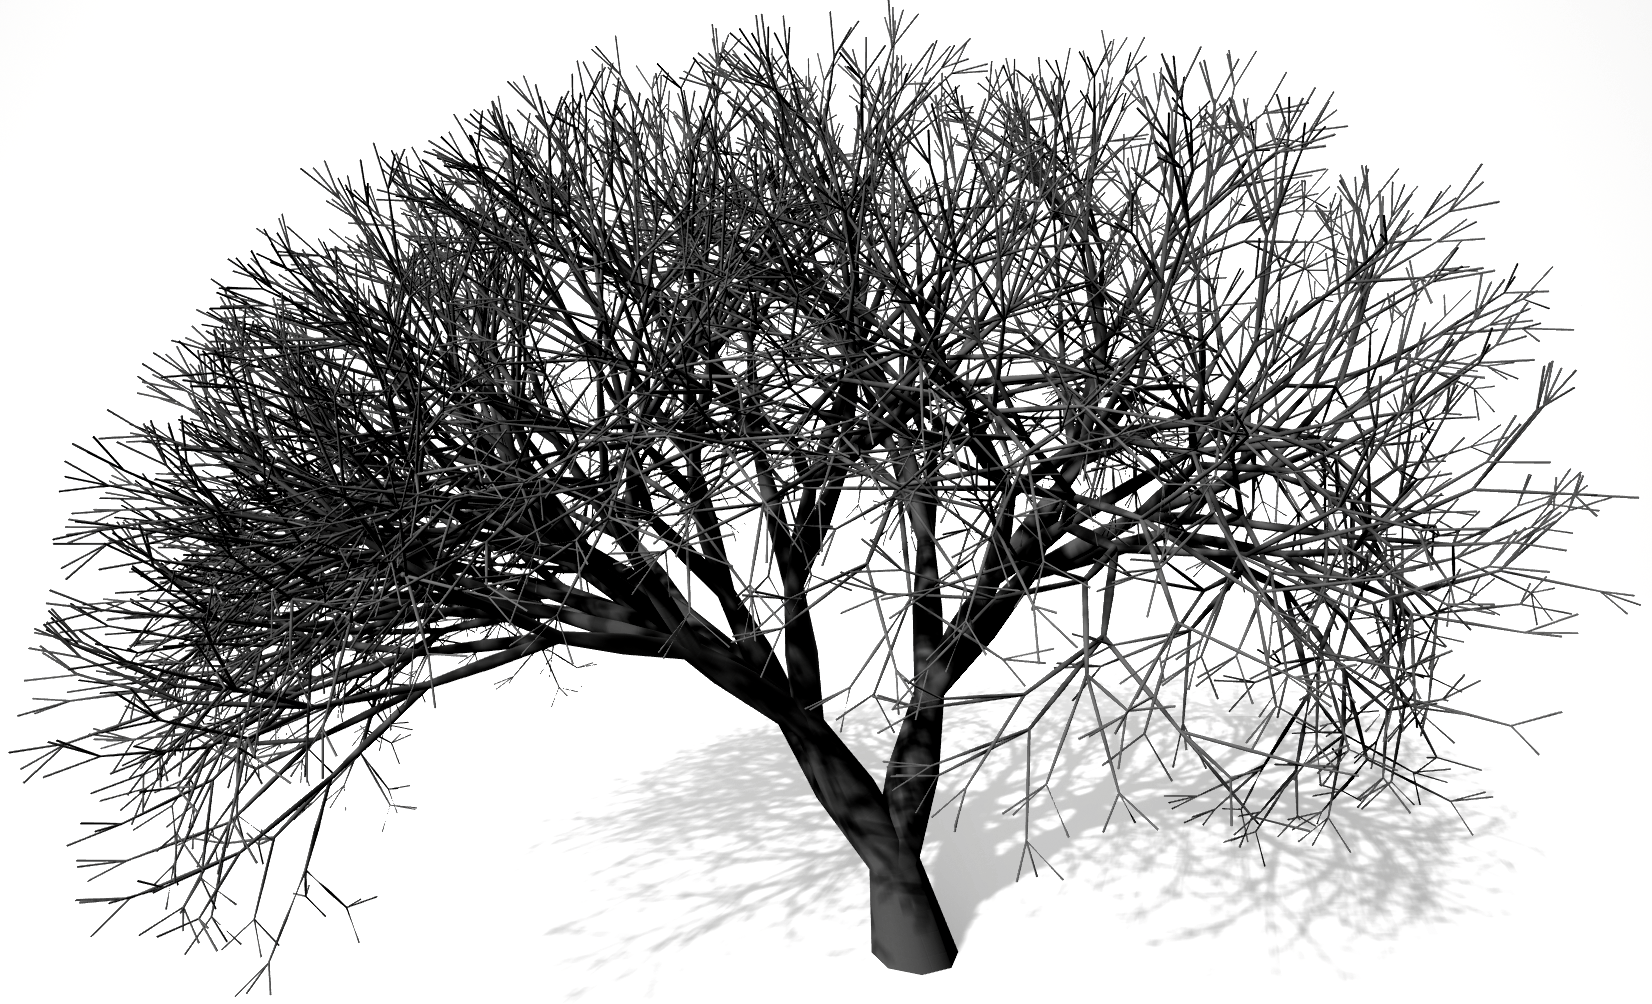
\includegraphics[height=.19\textheight]{images/Performance_LS_Ternary_4_Tropism.png}
		\caption{Ableitung anhand Gleichung \ref{eq:ProdTernary} entsprechend den Werten aus Abbildung \ref{subfig:LS_Ternary_4_Tropism}. \\ $n_{min} = 8$, $n_{max} = 8$, $max_K = 1.0$, \\ $\text{Generierungszeit}= 0.233s$, $206658 \text{ Vertizes}$.}
		\label{subfig:Performance_LS_Ternary_4_Tropism}
	\end{subfigure}	
	\caption{Vergleich von Generierungszeit und resultierender Datenmenge zwischen L-System-Actor und Space-Colonization-Actor. Eigene Abbildungen.}
	\label{fig:Results_ComparisonOfTime}
\end{figure}

Die Zeit, welche für die Generierung einer Baumstruktur durch den Space Colonization Algorithmus benötigt wird, stellt derzeit insbesondere für die Anwendung in digitalen Spielen ein Problem dar -- die Generierung einer einzigen, recht simplen Baumstruktur kann mehrere Sekunden beanspruchen. Die Generierungszeit ist jedoch stark abhängig von der Anzahl an Einflusspunkten, der Schrittweite sowie der maximalen Iterationsanzahl und kann somit von einem Benutzer eingeschätzt und angepasst werden. Weiterhin bietet die vorgestellte Implementierung Potenzial für zukünftige Erweiterungen, welche eine Verminderung der Generierungszeit als Ziel haben.

Die durch den Space Colonization Algorithmus generierte Datenmenge lässt sich durch eine Vielzahl von Parametern beeinflussen -- insbesondere unter Verwendung der implementierten Kurvenreduktion kann die Datenmenge eines Baummodells verringert werden, ohne die Baumstruktur visuell stark zu beeinträchtigen.

\subsection{Benutzerfreundlichkeit}

Für die Verwendung eines L-System-Actors muss der Benutzer eine genaue Vorstellung über den Aufbau der zu generierenden Baumstruktur sowie Kenntnisse über die korrekte Definition von L-Systemen besitzen, um diese in Form von Axiomen, Produktionsregeln und Konstanten angeben zu können. Dies beansprucht ein gewisses Basiswissen über das Wachstumsverhalten von Bäumen sowie ein Verständnis für die entsprechende Umsetzung als L-System. \cite[S.86]{Deussen:05}

Bei der Verwendung eines Space-Colonization-Actors hingegen gibt es klare Zusammenhänge zwischen der Form einer Baumstruktur sowie den numerischen und Boolschen Parameterwerten, ohne dass ein tieferes Verständnis der Funktionsweise des Algorithmus erforderlich ist. Ein Benutzer kann immer wieder Parameter verändern, die Auswirkungen beobachten und weitere Änderungen durchführen, bis die gewünschte Baumstruktur generiert wurde. 
 \cite[S.89]{Deussen:05}
 
\section{Wünschenswerte Erweiterungen}

Die vorgestellten Implementierungen der gewählten Vorgehen bieten Potenzial für Verbesserungsmöglichkeiten, die in zukünftigen Arbeiten behandelt werden können.

\subsection{L-Systeme}

\paragraph{Konditionale L-Systeme}

In der von Prusinkiwicz u.a. vorgestellten Form fordern parametrische L-Systeme die Auswertung einer Bedingung vor der Ersetzung des parametrischen Wortes durch den Nachfolger. Die Bedingung bestimmt, ob die Ersetzung des Wortes durch den Nachfolger stattfindet. Konditionen sind nicht zwingend notwendig für die Generierung realistischer Baumstrukturen, würden dem Benutzer jedoch einen weiteren Kontrollmechanismus für die Gestaltung von Baumstrukturen bieten. Ein Benutzer könnte beispielsweise festlegen, dass nach einer vorgegebenen Anzahl von Ableitungen die Bildung großer, tragender Äste durch die Produktion kleiner Verzweigungen ersetzt wird. \cite[S.41f]{ABOP:04}

\paragraph{Stochastische L-Systeme}

Stochastische L-Systeme erweitern die Definition von Produktionsregeln um ein zufälliges Element und unterscheiden sich somit von der deterministischen Funktionsweise der vorgestellten L-Systeme. Demselben parametrischen Wort werden unterschiedliche Produktionsregeln und zugehörige Wahrscheinlichkeitswerte zugeordnet. Anhand dieser Werte wird zufällig bestimmt, welche der Produktionsregeln bei einer Ableitung des Wortes verwendet wird. Bei gleichbleibender L-System-Definition ergeben sich dadurch unterschiedliche Ergebnisse. Stochastische L-Systeme stellen somit eine Lösung von visuell unnatürlich wirkenden Regelmäßigkeiten in Baumstrukturen dar. \cite[S.28]{ABOP:04}

\paragraph{Benutzerfreundlichkeit}

Um die Verwendung von L-Systemen zu vereinfachen, können vordefinierte Wachstumsarten implementiert und durch den Benutzer mithilfe von numerischen Parametern anpassbar gemacht werden. Diese Erweiterung würde die intuitive Verbindung zwischen den Parametern und Veränderungen an der Baumstruktur erlauben, wird jedoch durch die Anzahl der vordefinierten Wachstumsarten limitiert. Um diesem Problem entgegenzuwirken, könnte beispielsweise die Angabe von Anzahl, Länge und Abzweigungswinkel von Verzweigungen in dem Nachfolger einer Produktionsregel mithilfe von numerischen Parametern ermöglicht werden. Aus den eingegebenen Informationen werden daraufhin die entsprechenden Produktionsregeln automatisch definiert.

\paragraph{Einsatz vordefinierter Modelle}

Die Möglichkeit benutzerdefinierte Zeichen durch vordefinierte 3D-Modelle zu ersetzen würde den Einsatz von Blüten, Blättern oder anderer Strukturen im Baummodell ermöglichen. Aufgrund der Selbstähnlichkeit von, durch L-Systeme generierten, Baumstrukturen besteht ebenfalls die Möglichkeit einen Teilbaum des graphentheoretischen Baums in mehreren Rotationen und Positionen wiederzuverwenden um somit den benötigten Interpretationsaufwand zu verringern. \cite[S.82]{Deussen:05}

\subsection{Space Colonization Algorithmus}

\paragraph{Positionsabfragen}

Ungefähr $90\%$ der Generierungszeit, die für einen Space-Colonization-Actor benötigt wird, entsteht bei der Überprüfung, welche Astsegmente sich innerhalb des Einflussradius eines Einflusspunktes befinden. Derzeit wird jede Position eines Punktes mit jeder Endposition eines Astsegments verglichen. Es gibt einige Möglichkeiten eine solche Brute-Force-Methode zu verbessern, beispielsweise durch die Verwendung von Octrees. Diese stellen eine Methode dar, dreidimensionalen Raum in Form eines graphentheoretischen Baumes aufzuteilen um somit die Anzahl von benötigten Positionsabfragen zu reduzieren. \cite[S.1]{Octree:10}

\paragraph{Einflussbereiche} 

Die derzeit implementierte Möglichkeit Einflussbereiche anzugeben ist begrenzt auf die Definition von Primitiven in Form von Kugeln und Zylindern. Werden mehrere Primitive als Einflussbereiche miteinander kombiniert, gibt es keine Möglichkeit die Punkteverteilung in sich überschneidenden Bereichen zu normalisieren. Eine Erweiterung der Primitive um Rechteck-, Kegel- und Pyramidenformen sowie die Möglichkeit, Bereiche zu definieren, in welchen keine Einflusspunkte generiert werden, würden die Gestaltungsmöglichkeiten der generierbaren Baumstrukturen verbessern. 

Die Anpassung der Verteilung von Einflusspunkten innerhalb der Einflussbereiche stellt eine zusätzliche Erweiterung dar. Runions u.a. zeigen, dass die ausschließliche Platzierung von Punkten auf der Oberfläche eines Einflussbereichs oder das dynamische Hinzufügen von Punkten in jeder Iteration des Algorithmus die Generierung zuvor unmöglicher Baumstrukturen zulässt. \cite[S.5f]{ABOP:04}

\subsection{Allgemeine Erweiterungen}

Die folgenden Vorschläge befassen sich mit Erweiterungen, welche sich auf alle generierten Baumstrukturen beziehen.

\paragraph{Generierung zur Laufzeit}

Im Bereich der Echtzeitanwendungen ist die Zeit, welche für den Start einer Anwendung aufgebracht wird, limitiert. Die Anzahl von Baumstrukturen, welche in einer solchen Zeit generiert werden können ist begrenzt. Eine Möglichkeit dieses Problem zu umgehen ist, die Baumstrukturen während der Laufzeit zu generieren. Beispielsweise könnte sich ein Spieler bereits im Level bewegen, während um ihn herum Baumstrukturen nach ihrer Fertigstellung dargestellt werden. Das resultierende, plötzliche Auftauchen von Objekten ist ein Nachteil, der gegen den Vorteil einer verringerten Ladezeit abgewägt werden muss.

\paragraph{Level-of-Detail (LOD)}

Je weiter ein 3D-Modell vom Beobachter entfernt ist, desto kleiner erscheint es auf dem Bildschirm. Eine komplexe Baumstruktur ist dann nicht mehr von einem Baummodell mit reduzierter Datenmenge unterscheidbar. Die derzeitige Implementierung stellt, unabhängig von der Entfernung, alle Modelle mit derselben Datenmenge dar. Unterschiedlich komplexe Modelle einer Baumstruktur -- die LOD-Qualitätsstufen des Modells -- können in Abhängigkeit von der Entfernung zum Beobachter dynamisch ausgetauscht werden. Dadurch wird die, in jedem Frame darzustellende, Datenmenge reduziert. \cite[S.267]{Deussen:05}

\paragraph{Visuell}

Den generierten Baumstrukturen fehlen zwei ausschlaggebende Merkmale von Bäumen: Die Darstellung von Baumrinde und Blättern. 

Die Oberflächenbeschaffenheit der Strukturen kann derzeit lediglich durch Angabe eines Materials durch den Benutzer selbst beeinflusst werden. Die Möglichkeit prozedural generierte Texturen zu verwenden, welche Baumrinde simulieren, würde jedoch eine wünschenswerte Erweiterung darstellen. 

Die Blattform und ihre Verteilung stellen grundlegende, charakteristische Merkmale von laubtragenden Bäumen dar. Die Angabe von Blattformen durch Benutzer oder die prozedurale Generierung sowie Verteilung auf einer Baumstruktur wäre somit ebenfalls eine Erweiterung, welche in zukünftigen Arbeiten behandelt werden könnte.

\paragraph{Verteilung}

Die derzeit generierten Baumstrukturen müssen einzeln in einem Level platziert und ihre Parameter festgelegt werden. Dies ist für eine kleine Szene oder die Platzierung von wenigen Bäumen an bestimmten Positionen praktikabel, nicht jedoch für Szenen mit hunderten von darzustellenden Bäumen. Die Verteilung von Baumstrukturen in einer Szene, durch vollständig prozedurale Methoden oder mit Benutzerbeteiligung wäre eine wünschenswerte Erweiterung. Ein Benutzer könnte beispielsweise bestimmte Wachstumsbereiche angeben, in welchen vorgegebene Baumarten mit zufälligen Parametern platziert werden. 
